% !TeX root = ../main.tex
% -*- coding: utf-8 -*-

\chapter{基于相关统计量的缺陷定位}
本章的研究内容主要针对一种重要的纠错性软件维护手段--缺陷定位。本章首先描述了缺陷定位对维护软件正确性
的作用,然后描述了基于程序谱的缺陷定位方法的一般过程。针对程序中可能存在多错误的问题,本文提出了基于
相关统计量的可疑度计算方法,在计算过程中尽可能避免多错误之间的相互影响。接着阐述了实验评估部分,描述
了实验设置,包括实验对象、对比实验和评价指标。在展示了实验结果和分析之后,对本章进行小结。

\section{引言}
软件系统在当今社会的军事、生活、教育等各个方面占据着重要的地位。随着人们对软件系统依赖性的不断增强,
软件系统失效往往给生活和经济带来巨大的损失,尤其在军事、航空等对可靠性有高要求的行业。软件缺陷是导致
软件失效的主要因素。软件缺陷的存在可能导致软件系统不能按照预期执行,从而造成误差甚至系统崩溃。为了保
证软件正确性,需要软件维护人员及时清除可能导致软件失效的缺陷。

当软件系统失效时,需要对软件系统进行纠错性软件维护,将潜在的软件缺陷清除。缺陷定位指的是当软件失效
时,查找并定位软件缺陷的过程,是纠错性软件维护的基础。虽然缺陷定位是纠错性软件维护的首要条件,但是人
工进行缺陷定位往往是一个冗长而繁复的过程。一方面人工缺陷定位通常依赖软件维护人员的经验和对软件系统的了解,
即使经验丰富的软件维护人员也很难迅速定位导致软件系统行为失效的根本原因。另一方面,针对大规模软件系统,人工缺陷定位所消耗的时间较长,软件维护人员需要充分理解源代码后逐步排查。

为了帮助软件维护人员查找缺陷,研究者们在自动缺陷定位的研究上投入了大量的工作。当前主要的缺陷定位方法
包括基于覆盖分析的方法、基于程序切片的方法、基于程序不变量的方法、基于模型检验的方法、基于状态变更的
方法等。其中大多数方法通过对软件系统的源代码或行为进行建模,查找与软件系统失效的代码。根据建模对象的
不同,传统的缺陷定位方法可以分为动态分析和静态分析两类。前者通过动态分析程序的行为,如执行路径或状态
等,查找相关代码;后者主要通过静态分析软件系统的源代码,从而分析与软件系统失效行为有关的程序元素。虽
然自动化缺陷定位的理论和技术得到了很大的发展,但当前的自动缺陷定位仍然面临两个挑战:

\begin{itemize}
      \item 随着需求的不断增加,软件系统越来越大,导致缺陷定位的效率降低。因此,适用于大规模软件系统的
   的缺陷定位越来越得到关注。
      \item 软件系统中潜在的缺陷可能不止一个,多个软件缺陷之间的相互影响可能导致自动缺陷定位的难度提
      高,准确度下降。尽管目前已经存在部分针对多缺陷的调试技术,但多缺陷的自动定位仍然是不小的挑战。
\end{itemize}

基于覆盖分析的缺陷定位方法,其核心思想是被失效用例执行越多、成功用例执行越少的代码可疑度越高。该类方
法通常只需要统计测试用例的执行结果和覆盖信息,并根据特定的公式计算代码的可疑度,不需要对软件系统的源
代码进行建模,因此计算复杂度低,在面对大规模软件系统时效率较高。然而,引起测试用例失效的软件缺陷可能
不止一个,忽略不同软件缺陷之间的相互影响,可能导致缺陷定位的准确性降低。其主要原因有两个方面:(1)
未被失效用例覆盖的代码可能也包含缺陷;(2)不同软件缺陷共同路径上的正确代码被失效用例覆盖的频率较
大,导致可疑度偏高。本文引入相关统计量的概念,通过将测试用例执行的覆盖信息作为特征,测试用例执行结果
作为标签,将原问题转化为数据挖掘问题,从而推测特征(代码)对执行结果的重要性。

本章具有以下贡献:
\begin{itemize}
      \item 本章提出了基于相关统计量的缺陷定位方法,从数据的角度分析测试用例的覆盖信息,利用特征选择
中特征对分类结果重要性的概念,将对测试用例执行结果影响较大的代码的可疑度提高。
      \item 该方法在传统的基于覆盖分析的缺陷定位方法上引入了相关统计量,同样不需要对源代码进行建模,计算复杂度较低。
      \item 针对多缺陷之间相互影响的问题,相关统计量为每个测试用例选择距离最近的同类和异类样本,计算
      测试用例在每个特征上距离同类和异类的距离,从而计算特征对测试执行结果的重要性。该方法在很大程度
      上避免了在衡量特征重要性时多错误之间的相互影响。
      \item 在开源软件系统上的实验证明,本章方法相比较传统启发式的基于覆盖分析的缺陷定位方法在准确性
      上具有一定的提升,通过提高缺陷查找效率缩短了纠错性维护的时间和人力成本。
\end{itemize}

\section{研究动机与相关工作}
传统的基于覆盖分析的缺陷定位方法,基于启发式的思想使用特定公式计算程序元素的可疑度,其优点在于计算复
杂度低,面对大规模软件系统的效率较高,但也存在一定的问题:由于基于覆盖分析的方法不对程序源代码进行建
模,而是从统计的角度根据代码被失效和成功覆盖的频率推测代码的可疑度,因此对于存在多错误的失效用例,难
以区分不同缺陷导致的失效用例,而缺陷之间的相互影响是导致多缺陷定位的准确性下降的主要原因。

\subsection{研究动机}
\begin{figure}[htp]
      \centering
      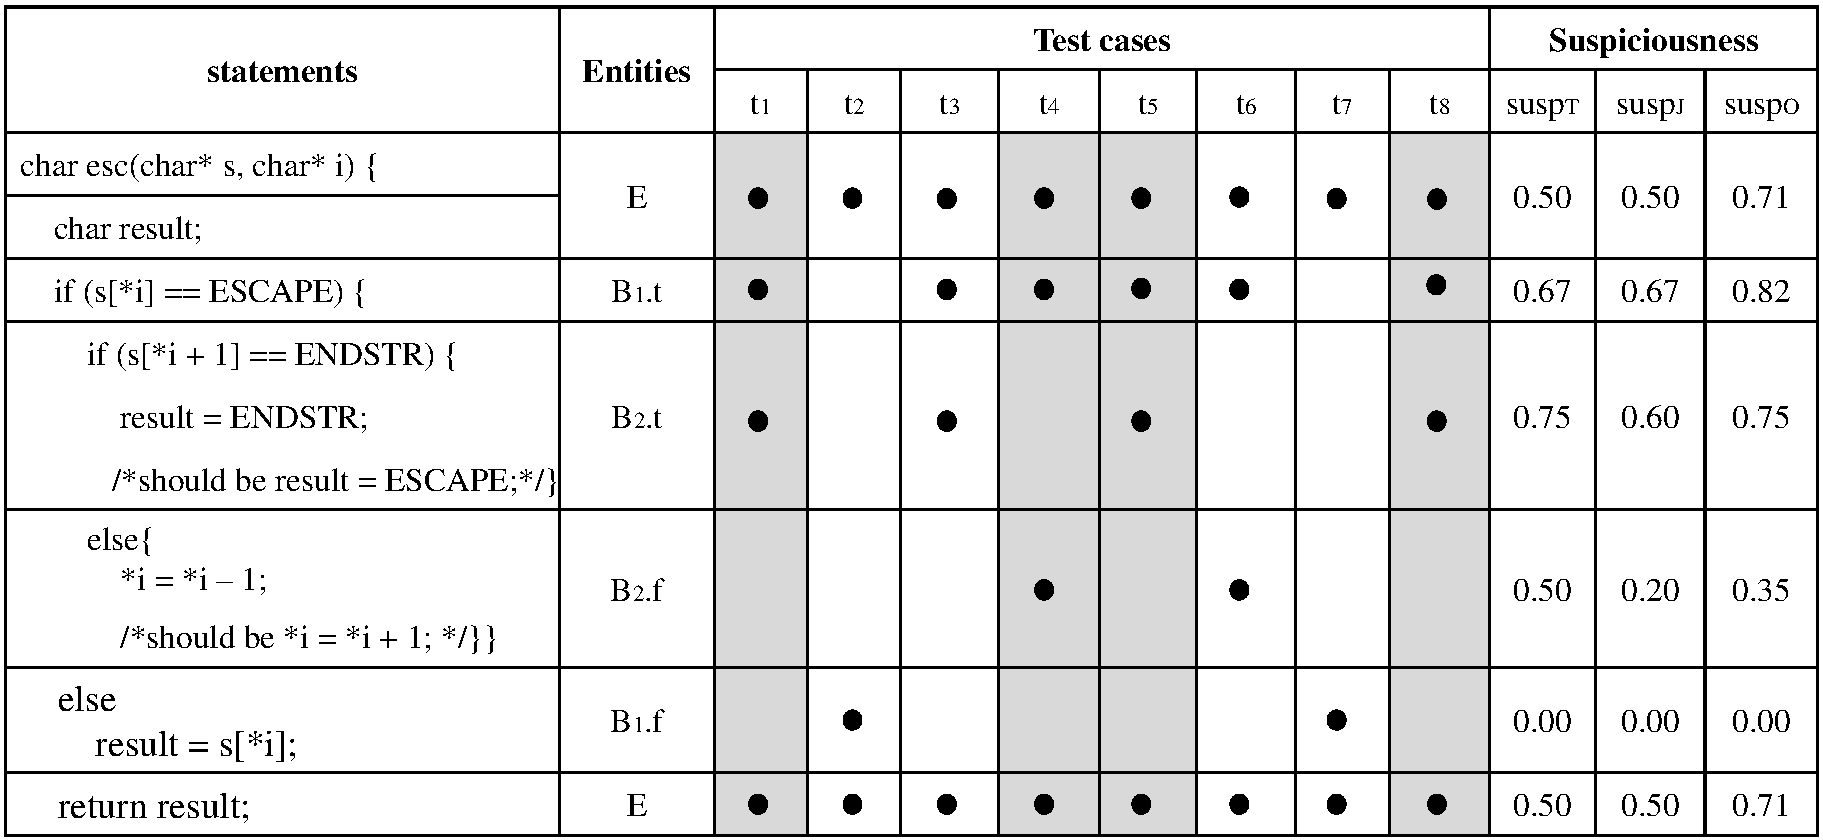
\includegraphics[width=0.95\linewidth]{spectra.pdf}
      \caption{示例程序的分支覆盖特征谱}
      \label{fig:spectra}
\end{figure}

图~\ref{fig:spectra}是示例程序的分支覆盖特征谱,示例代码来自于西门子标准集
\footnote{http://sir.unl.edu/portal/index.php}。图~\ref{fig:spectra}中的示例代码共有2个嵌套的分支结
构,分别是$B_1$和$B_2$。对于每个分支结构,我们用分别用$t$和$f$来示意其两个分支,如$B_1.t$表示第一个
分支结构的真分支。根据分支情况将示例代码分为五个部分,可表示为$P = \{E, B_1.t, B_1.f, B_2.t,
B_2.f\}$,其中$E$表示程序的入口代码快。图~\ref{fig:spectra}中共有8个测试用例,每个测试用例的覆盖信息
表示为一列,黑色圆圈表示该测试用例覆盖了所对应的程序元素。灰色阴影的测试用例表示该用例的执行结果为失
效;反之则为成功用例。右边三列表示用三种经典的可疑度计算公式计算出的可疑度,分别是
Tarantula~\cite{jones2005empirical}、Jaccard~\cite{abreu2007accuracy}和
Ochiai~\cite{abreu2007accuracy}。

以图~\ref{fig:spectra}中的示例代码为例,该代码片段中存在两个缺陷$d_1$和$d_2$,分别在分支结构$B_2$的
真假分支$B_2.t$和$B_2.f$上。失效用例集为$T_f=\{t_1, t_4, t_5, t_8\}$,其中测试用例$t_1, t_5, t_8$覆
盖$d_1$,用例$t_4$覆盖$d_2$。由图~\ref{fig:spectra}可以看出,由于示例代码存在两个缺陷,导致对于每个
缺陷,都存在不覆盖该缺陷的失效用例。例如对于缺陷$d_2$,虽然被失效用例$t_4$覆盖,但是由于缺陷$d_1$的
存在,导致大多数失效用例都不需要覆盖缺陷$d_2$,因此按可疑度比实际偏低。图~\ref{fig:spectra}中的三个
可疑度计算结果可以看到,分支$B_2.f$的可疑度远远比$B_2.t$低,甚至比$E$的可疑度更低。值得注意的是,由
于分支$B_1.t$存在于两个缺陷的共同路径上,因此其被所有的失效用例覆盖,导致其可疑度比实际偏高。

为了说明缺陷个数和基于覆盖分析的可疑度计算之间的关系,本文用$\alpha$表示其被失效用例覆盖的次数占失效
用例总数的比例。当程序中只存在一个缺陷$d$时,所有失效用例均覆盖该缺陷,因此不存在未覆盖该缺陷却导致
测试用例失效的情况,$\alpha=1$永远成立;而当程序中存在不止一个缺陷时,导致测试用例失效的缺陷可能不止
一个,覆盖其中一个或多个缺陷的测试用例都有可能会触发缺陷,导致软件行为失效,因此可能存在失效用例只覆
盖其中部分缺陷,此时$\alpha<=1$;随着具有破坏程序行为能力的缺陷个数越来越多,每个缺陷所触发的失效用
例占失效用例总数比例越来越小,此时$\alpha$也随之变小。

以Tarantula\cite{jones2005empirical}为例,使用$\alpha$可将公式~\ref{eq:tar}表示为:
\begin{eqnarray}
 susp_T = \frac{1}{1+\frac{|T_p|}{\alpha}}, \label{eq:t}
\end{eqnarray}
其中$|T_p|$表示成功用例的个数。从公式~\ref{eq:t}中可以看出,随着软件中包含的缺陷越来越多,由于每个缺
陷所导致的失效用例占总失效用例的比例下降,导致包含缺陷的程序元素所对应的$\alpha$变小,因此缺陷的可疑
度$susp_T$降低,从而影响了缺陷定位的准确度和效率。

\subsection{多缺陷定位相关工作}
在早期研究中,有研究者提出``One-bug-at-a-time''~\cite{klahr1988cognitive},将多缺陷程序视为单缺陷程
序进行定位,在修复缺陷后若还存在失效用例,则继续缺陷定位并修复。这种方法由于忽略了缺陷之间的相互影
响,导致定位缺陷的准确率较低,且由于需要重复执行测试用例集,因此效率较低。

一种理想的解决方式是将由不同缺陷导致的失效用例划分成为不同的失效用例集,对其中每个失效用例集可视为当
前程序只存在一个可触发程序失效的缺陷,其余缺陷均不能引起程序行为失效。在这种情况下,所有失效用例均覆
盖包含缺陷的代码,此时缺陷代码的$a_{01}=0$,因此$\alpha$取得最大值。根据公式~\ref{eq:t}可知,当
$\alpha$取最大值时,缺陷代码的可疑度最高。这种方法的优点在于每个失效用例集均来自于同一缺陷,因此测试用例的直观性比较强,使用单缺陷定位方法能够快速定位到缺陷。

为了达到这个效果,部分学者使用聚类分析将失效用例进行聚类~\cite{jones2007debugging,
zheng2006statistical},对每类失效用例采用单缺陷的方法进行处理。基于聚类分析的方法,其核心思想是由相
同缺陷引起的失效用例其程序行为相似,具有相似的覆盖信息。这种方法虽然在一定程度上提高了多缺陷的定位准
确率,但是依赖聚类分析的准确性,很难完全避免多缺陷之间的相互影响。

文万志等人~\cite{conslice2013}提出使用条件切片进行多缺陷定位,该方法根据输入条件的不同计算出不同的条
件切片,将失效用例进行划分,每类失效用例被视为由同一缺陷引发,最后通过基于覆盖分析的缺陷定位技术计算
可疑度。该方法与基于聚类分析的方法类似,其最终目的是将多缺陷程序当做单缺陷程序处理,在依赖划分准确性
的同时忽略了缺陷之间的相互影响;与之不同的是,本文方法不需要对失效用例进行划分,且不需要进行条件切
片。

基于失效用例划分的多缺陷定位方法~\cite{zheng2006statistical, jones2007debugging, conslice2013}虽然在
一定程度上提高了多缺陷定位的效率,但其准确度依赖于失效用例划分的质量。不准确的划分使得同一失效用例集
中包含来自多个缺陷的失效用例,因此容易导致混入由其它缺陷导致的失效用例,从而引入噪音;除此以外,由于
划分导致每个失效用例集的规模变小,因此可能引起缺陷定位的不准确性。

何加浪等人~\cite{neural2013}提出使用神经网络定位多缺陷,该方法通过学习输入和缺陷之间的关系,计算代码
的各个位置与每个缺陷之间的相关性来定位缺陷。该方法利用神经网络的泛化能力学习代码和缺陷的相关性,需要
提前假定程序中的缺陷个数。而在实际应用中,软件维护人员很难提前知道潜在的缺陷个数。与之不同的是,本文
方法对缺陷个数不敏感,无需假定程序中存在的缺陷个数,且计算复杂度较低,更适用于大规模软件系统。

\section{基于相关统计量的缺陷定位算法}
本章在基于覆盖分析的缺陷定位技术的基础上引入了相关统计量的概念,从数据挖掘的角度计算代码对程序执行结
果的重要性,通过为每个测试用例寻找距离最近的测试用例,在很大程度上避免了多缺陷相互之间的影响,提升了
缺陷定位的效率和准确率。

\subsection{基于覆盖分析的缺陷定位}
\begin{figure}[htp]
      \centering
      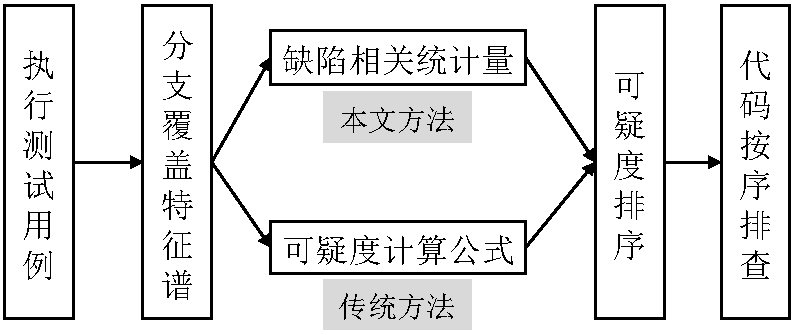
\includegraphics[width=0.6\linewidth]{fault_flow.pdf}
      \caption{基于相关统计量的方法}
      \label{fig:fault_flow}
\end{figure}

本文在基于覆盖分析的缺陷定位技术通过执行测试用例,统计测试用例执行过程中的覆盖信息和执行结果,最后根
据特定的可疑度计算公式逐个计算每个程序元素的可疑度,并按照可疑度由高至低排查对应代码。以分支覆盖特征
谱为例,如图~\ref{fig:fault_flow}所示,本文的缺陷定位过程主要包括以下三步:
\begin{itemize}
     \item 运行测试用例,收集测试用例运行过程中的分支覆盖信息,得到分支覆盖特征谱矩阵;
     \item 计算每个分支与程序结果之间的相关统计量,结合经典的可疑度计算公式计算可疑度;
     \item 按照可疑度大小由高至低推荐给软件维护人员进行逐个排查。 
\end{itemize}

\begin{Definition}
      程序。程序$P$由代码表示,记作$P=\{e_1, e_2, e_3, ..., e_n\}$,其中$e$表示特定的
      程序元素。
\end{Definition}

为了收集测试用例执行的覆盖信息,首先将程序表示为由程序元素组成的序列。常用的程序元素有语句、分支、谓
词、定义对等。根据元素的粒度不同,可以将程序元素分为语句和基本块两类,前者将程序的所有语句表示成一个
序列,记录每条语句的覆盖信息;后者将程序表示为基本块序列,每个基本块由部分程序语句组成(如分支等)。
程序元素可以是基于控制流的程序语句组合(如语句、分支等),也可以是通过数据流分析提取的变量的定义-使
用对,通过关注在成功和失效用例中变量的使用情况来定位缺陷,还可以是其它与程序行为相关的关键代码,如谓
词等。程序元素的多样性使得基于覆盖分析的缺陷定位技术更加灵活和高效。

\begin{Definition}
      软件缺陷。软件缺陷是程序中存在的对程序行为具有破坏能力的错误或功能缺陷,记作$d$。
\end{Definition}

\begin{Definition}
      成功用例。执行测试用例,当且仅当程序$P$的输出与预期输出一致时,称该测试用例为成功用例,成功用
      例集记作$T_t$。
\end{Definition}

\begin{Definition}
      失效用例。执行测试用例,当程序$P$的输出与预期输出不一致时,称该测试用例为失效用例,失效用例集
      记作$T_f$
\end{Definition}

软件缺陷是导致程序行为与预期不同的主要原因,纠错性软件维护通过查找和修复软件缺陷,提高软件系统的可靠
性。根据测试用例执行的结果是否与预期一致,可以将测试用例集划分为成功用例和失效用例两类。成功执行的测
试用例可能未覆盖软件缺陷,也可能覆盖但并未出发软件缺陷;相反,失效执行的测试用例覆盖并触发至少一个软
件缺陷,导致程序的正常行为被破坏,与预期不一致。

\begin{Definition}
      程序谱。给定程序$P$和测试用例集$T$,程序谱用来记录测试用例集$T$对程序$P$在执行过程中的覆盖信
      息,记作二维矩阵$S_{m\times n}$,其中$m$表示测试用例集的规模,$n$为程序中所含程序元素的个数。
      矩阵元素$S_{ij}$为
      \begin{eqnarray}
         S_{ij} = \begin{cases} 1, & \mbox{第}i\mbox{个测试用例覆盖了第}j\mbox{个程序元素} \\ 
  0, & \text{ 其它 }  
  \end{cases}   , 1 \leqslant i \geqslant  m, 1 \leqslant j \geqslant n
      \end{eqnarray}
\end{Definition}

在确定程序元素后,通过插桩技术记录测试用例执行过程中是否覆盖特定的程序元素,并将结果记录在程序谱
中。需要注意的是,程序谱只记录程序元素的是否被测试用例覆盖,并不记录测试用例执行的顺序,因此程序谱通
常是二维0-1矩阵,其所占内存与测试用例集的规模和程序规模有关,通常在可接受范围内。

\subsection{Relief特征选择模型}

缺陷定位的目的是查找引起程序行为失效的程序代码。不考虑外部因素,失效用例的执行路径一定覆盖一个或多个
软件缺陷,而不覆盖软件缺陷的测试用例一定是成功用例。因此,是否执行缺陷代码与程序行为是否失效两者之间
存在一定的相关性。本文假设是否覆盖缺陷代码是判断程序行为是否失效的重要因素,借鉴特征选择中的相关统计
量概念计算代码对程序行为结果的重要性,从而定位软件缺陷。

给定程序$P$,测试用例集$T$中的每个测试用例可视为一条样本数据。将测试用例对代码的覆盖情况作为该测试用
例的特征,根据测试用例的执行结果对其进行标记,成功用例被标记为正类、失效用例被标记为负类。测试用例集
中第$i$个测试用例可通过$T_i=\{x_{i1},x_{i2},x_{i3},...,x_{in}\}$来表示,其中$n$为程序中所含语句或分
支的个数,$x_{ij}$表示测试用例$T_i$是否覆盖第$j$个程序元素(覆盖为1,不覆盖为0)。




Relief算法最早由Kira提出,最初局限于两类数据的分类问题。Relief算法是一种特征权重算法(Feature
weighting algorithms),根据各个特征和类别的相关性赋予特征不同的权重,权重小于某个阈值的特征将被移
除。Relief算法中特征和类别的相关性是基于特征对近距离样本的区分能力。算法从训练集D中随机选择一个样本
R,然后从和R同类的样本中寻找最近邻样本H,称为Near Hit,从和R不同类的样本中寻找最近邻样本M,称为
NearMiss,然后根据以下规则更新每个特征的权重:如果R和Near Hit在某个特征上的距离小于R和Near Miss上的
距离,则说明该特征对区分同类和不同类的最近邻是有益的,则增加该特征的权重;反之,如果R和Near Hit在某
个特征的距离大于R和Near Miss上的距离,说明该特征对区分同类和不同类的最近邻起负面作用,则降低该特征的
权重。以上过程重复m次,最后得到各特征的平均权重。特征的权重越大,表示该特征的分类能力越强,反之,表
示该特征分类能力越弱。Relief算法的运行时间随着样本的抽样次数m和原始特征个数N的增加线性增加,因而运行
效率非常高。具体算法如下所示:

具体来说,Relef为每个测试用例寻找距离最近的同类和异类样本,距离同类越近、距离异类越远的特征
被认为越能够区分不同类别的样本。

具体算法

\subsection{面向缺陷定位的相关统计量}
\subsubsection{(2)可疑度计算}

\subsection{代码排查}
The principle to map a branch or function element that is with high suspiciousness to the
corresponding code is as below: (1) If the element is one branch of the branch structure, go to (2);
else go to (5). (2) Check the corresponding branch structure judgment of this branch. (3) Check the
executable code which probably have infect on the judgment result in the basic block where the above
judgment is. (4) Check control dependent on executable code of this branch, which means whether this
branch executed or not determines whether this part of executable code execute or not, after the
check turn to (6). (5) It is time to check the function coverage feature elements. Check all
executable code that must execute in the functions, including the judgments of partial branch
structure. (6) Order the results by suspiciousness, check next feature elements. Taking branch in
Fig. 1 as example, according to step (2), firstly check judgment of the branch structure which this
branch is in, namely the fifth line code; Since there is no executable code which can influence the
judgment result and located in the same basic blocks with this fifth line code, step (3) is passed
over; Finally check the code of control independent on branch B2.f, namely sentence nine (including
other branches judgments)

\section{实验设置}
\subsection{实验对象}

\subsection{对比实验}
使用三种经典的可疑度计算方法,分别是Tarantula~\cite{jones2005empirical}、
Jaccard~\cite{abreu2007accuracy}和Ochiai~\cite{abreu2007accuracy},可疑度计算公式如下:
\begin{eqnarray}
 susp_T = \frac{\frac{a_{11}}{a_{11}+a_{01}}}{\frac{a_{11}}{a_{11}+a_{01}}+\frac{a_{10}}{a_{10}+a_{00}}}, \label{eq:tar}\\
susp_J = \frac{a_{11}}{a_{11}+a_{01}+a_{10}}, \label{eq:jac}\\
susp_O = \frac{a_{11}}{\sqrt{(a_{11}+a_{01})\times(a_{11}+a_{10})}}, \label{eq:och}
\end{eqnarray}

上述公式中的四个变量均用来描述程序元素覆盖与否信息与执行结果之间的关系:
\begin{itemize}
  \item $a_{00}$表示测试用例被成功执行但未覆盖某个程序元素;
  \item $a_{01}$表示测试用例执行失效且未覆盖某个程序元素;
  \item $a_{10}$表示测试用例被成功执行且覆盖某个程序元素;
  \item $a_{11}$表示测试用例执行失效且覆盖了某个程序元素。
\end{itemize}

\subsection{评价指标}
\section{实验结果与分析}
\subsection{实验结果}
\subsection{结果分析}
\subsection{适用性讨论}
本以分支覆盖特征谱为例,提出了基于相关统计量的缺陷定位方法。值得注意的是,本章方法也同样适用于其它
程序元素。
依赖测试用例集的质量。如果特别不平衡的话,还是容易导致某些缺陷被放大,某些缺陷被缩小。
\section{本章小结}
本章提出在覆盖分析的基础上使用相关统计量来定位缺陷,通过为每个测试用例选择距离其最近的同类和异类测试
用例,为每个失效用例找到最有可能与其由同一缺陷出发的失效用例。虽然基于相关统计量的缺陷定位与聚类分析
的方法是基于相似的核心思想,即由相同缺陷引起的失效用例具有一定的相似性,但本文方法在该思想的基础上加
了较大的约束,即本文认为只有距离失效用例最近的失效用例才可能由同一缺陷引起,因此在很大程度上避免了对
聚类分析准确性的依赖,且不需要聚类分析中的参数设置(如缺陷个数等参数)。

